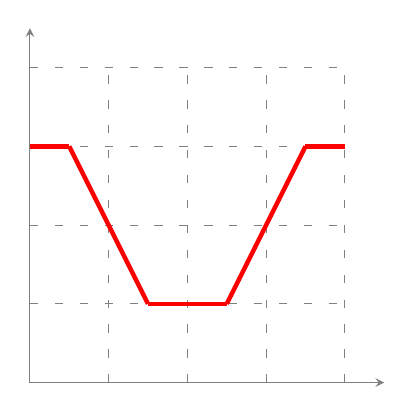
\begin{tikzpicture}[scale=1] % on multiplie les dimensions par 2
\draw[color=gray,thin,->,>=stealth] (0,0)--(4.5,0); % l'axe des abscisses
\draw[color=gray,thin,->,>=stealth] (0,0)--(0,4.5); % l'axe des ordonnées
\draw[color=gray,loosely dashed	]	(0,1)--(4,1);
\draw[color=gray,loosely dashed	]	(0,2)--(4,2);
\draw[color=gray,loosely dashed	]	(0,3)--(4,3);
\draw[color=gray,loosely dashed	]	(0,4)--(4,4);
\draw[color=gray,loosely dashed	]	(1,0)--(1,4);
\draw[color=gray,loosely dashed	]	(2,0)--(2,4);
\draw[color=gray,loosely dashed	]	(3,0)--(3,4);
\draw[color=gray,loosely dashed	]	(4,0)--(4,4);
\draw[color=red,ultra thick]		(0,3)--(0.5,3);
\draw[color=red,ultra thick]		(0.5,3)--(1.5,1);
\draw[color=red,ultra thick]		(1.5,1)--(2.5,1);
\draw[color=red,ultra thick]		(2.5,1)--(3.5,3);
\draw[color=red,ultra thick]		(3.5,3)--(4,3);
%\draw[color=gray] (1,-0.05)--(1,0.05) node[below=5pt] {$1$}; % le point (1,0)
%\draw[color=gray] (-0.05,1)--(0.05,1) node[left=5pt] {$1$}; % le point (0,1)
\end{tikzpicture}